% simple.tex - simple Master's thesis sample
% $Id: simple.tex 309 2011-01-28 14:46:48Z vlado $
\documentclass[12pt]{dalcsthesis}
% to prepare draft version use option draft:
%\documentclass[12pt,draft]{dalcsthesis}

\usepackage{algorithm2e}
\usepackage{graphicx}
\begin{document}
\mcs  % options are \mcs, \macs, \mec, \mhi, \phd, and \bcshon
\title{Feature Based adaptive motion model}
\author{Rohan Bhargava}
\defenceday{1}
\defencemonth{October}
\defenceyear{2013}
\convocation{January}{2014}

% Use multiple \supervisor commands for co-supervisors.
% Use one \reader command for each reader.

\supervisor{Dr. Thomas Trappenberg}
\supervisor{Dr. Mae Sato}
\reader{D. Odaprof}
\reader{A. External}
\providecommand{\tabularnewline}{\\}
\newcommand{\lyxdot}{.}
\nolistoftables
\nolistoffigures

\frontmatter

\begin{abstract}
We present a method to learn and adapt the motion model. The motion model can be influenced by environmental properties and is a crucial part of the navigation system.Examples are the drift that is accounted in the motion model can be different for carpets and tiles. The AUV can have a change in their motion model when they are moving from fresh water to sea water. Our algorithm is based on the Expectation Maximization Framework which help us to learn the right parameters for the model.
The Expectation Step is completed by particle filtering and smoothing. The Maximization step involves finding the parameters for the model.We use side sonar images to extract landmarks which can gives us position estimates to help us evolve our motion model.This leads to a better position estimate of the robot. 
We found that the our learning motion model adapted well to the change in parameters and had low localization error compared to static motion model. 
This algorithm eliminates the need for laborious and hand-tuning calibration process. The main significance of learning the motion model is to have better navigation algorithms and also its a step towards robots being able to adapt to environment without human intervention.
We validate our approach by recovering a good motion model when the density,temperature of the water is changed in our simulations. 
\end{abstract}

\begin{acknowledgements}
Thanks to all the little people who make me look tall.
\end{acknowledgements}

\mainmatter

\chapter{Introduction}
 





\section{Motivation}
The core of human environment interaction is the ability of the person to know its position in the surrounding environment. Similarly for robots the need to know its state in the world is an important task and it is termed as localization. To interact with the environment we need some sort of understanding of it.Primarily mapping the environment and localizing the robot in it i.e. Simultaneous Localization and Mapping (SLAM) has been a way to interact with the world. The integral part of SLAM is the way the robot moves and senses the world. The characteristics of movement and sensing the world are captured in the motion and sensor models. However infrequently discussed but essential input are the parameters to these models. Most of the models are considered to be static which is a wrong assumption to make. For example the movement of the robot on carpet is very different compared to tiles. Another example would be the models can change from general wear and tear on the robot. Generally the motion and sensor models are hand tuned by experts based on their experience. The whole process can be tedious and we propose a way to automate it. As we are moving ahead in our goal of making robots a ubiquitous part our everyday life they need to adapt to our dynamic surroundings. The algorithm that we are proposing not only will help automate the process but also help us adapt the models to our environment.

Water environments like oceans,rivers are highly dynamic and change in a matter of seconds which affects the movement of the vehicles.For example in Autonomous Underwater Vehicle(AUV) the density and the temperature of the water can lead to changes in the motion model. For my thesis we will specifically deal with underwater environments and propose an online system for an AUV to adapt its motion model. We specifically dealt with AUV that are equipped with side sonar sensor. 

Sound Navigation and Ranging (SONAR) is a technique based on sound propagation used for communication,detecting objects underwater. The SONAR sensor is the only imaging tool which can work at high depth. The side sonar images in my thesis is used for two applications. In the first application the side sonar images can be used to gather information for our sensor model. In second application by matching features on consecutive side sonar images we can get an estimate of the movement for the AUV. We use Speeded Up Robust Features(SURF) to extract interest points from the images. 

To learn the right parameters of the model we use Expectation Maximization(EM). It is an unsupervised machine learning technique primarily used to estimate parameters. It alternates between the Expectation Step which creates an expectation of the log-likelihood using the current estimate of the parameters and the Maximization Step which computes parameters maximizing the expected log-likelihood found in the E step. 

To summarize I am proposing a algorithm to learn the right parameters of the model specifically to deal with changes underwater. We are learning these parameters on the fly without having a prior map or revisiting places. We also put forward an idea to estimate the movement of AUV from side sonar images. Results of simulated experiments with environment changes are presented to show the effectiveness of the algorithm. Real mission datasets are used to validate our motion estimation algorithm. 
\section{Calibration and Localization}
\textbf{Localization} can be termed as the process of estimating the robot position and orientation in the world. It is the answer to the question “ Where am I?”. The correct estimate of its position is very crucial for the robot to achieve its goal. A erroneous estimate can lead to hazardous and fatal situations for the robot. Generally a prior map is provided and the robot is equipped with sensors to perceive the environment and localize itself in it. This process is an integral part in the autonomy of the robot. Various algorithms like Particle Filter, Kalman Filter help us in estimating the state of the robot in an environment. 

In our framework we use particle filters to localize the robot. We define a motion and a sensor model for our robot. Instead of a map we use dynamic landmarks to gather sensor readings. The motion and sensor measurements are then processed by particle filters to estimate the pose of the robot. 

\textbf{Calibration} is the process of determining the parameters to the kinematic or dynamical model. Better the calibration of the robot higher the accuracy of localization. Generally the robot is calibrated at the start of the experiment and the parameters values are not changed throughout the experiment. As our environment is dynamic our models whould also be adaptive.Thrun first proposed an algorithm for online calibration using the maximum likelihood estimate. Alziar further continued the work and learned the motion model for land robots using Expectation Maximization framework. The EM framework was further extended by Teddy Yapp to learn the right parameters for motion as well as sensor model. 

As stated earlier underwater environment is highly dynamic.Therefore we use the same framework to estimate the motion models for underwater vehicles. We use side sonar images to extract landmarks and use it as our sensor data. Particle smoothing is performed to get us a set of trajectories. We perform maximum likelihood estimate of the parameters given the trajectories and actual data. 

\section{General Architecture}


\begin{figure}[hbtp]
\caption{Block Diagram of the framework}
\centering
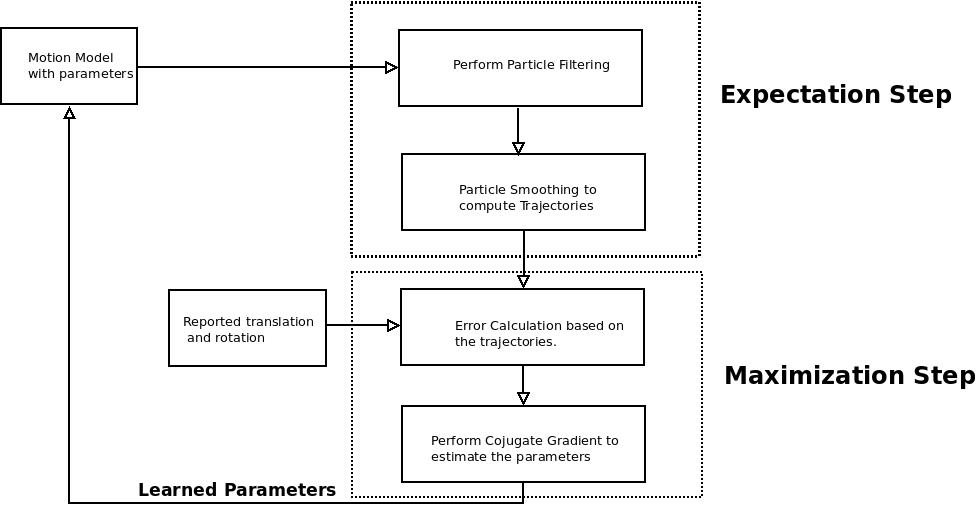
\includegraphics[scale=0.5]{Diagram1.jpeg}
\end{figure}



Figure 1.1 is a block diagram describing the whole system. The
first step is to initialize the motion model with a set of parameters.
Then the motion model is used to perform particle filtering which
is described in detail in the next chapter. The output of this step
is a set of particles with their importance weights.Particle smoothing
is performed on these set of particles. This gives us a collection
of trajectories and completes the Expectation step. 

Based on the trajectories and the reported translational and rotational
motion we calculate errors at each time step. We perform newton conjugate
gradient on the errors to give us the best estimate of the parameters.
This completes the Maximization Step.

The learned parameters are assigned to the motion model and the whole
process is repeated at each time step. The whole algorithm gives us
a model which can adapt to dynamic environment. The adaptive motion
model performs better than the static and the results are shown in
the later chapters.

\section{Motion Estimation}
In mobile robots the position and orientation is determined through wheel encoders and velocity estimates. These techniques do not generalize well as they cannot be applied to every robot. On top of that the wheels tend to slip on the floor and also the estimates drift over time. As the errors accumulate, the motion estimation becomes unreliable. 
We propose a method to estimate motion from only side sonar images.Compared to other techniques they are not restricted to particular locomotion method as well as don't suffer from drift.In our approach we extract and map key points between consecutive image in underwater environment . We use Speeded Up Robust Features (SURF) algorithm first proposed by Herbert Bay in 2006 to extract interest points in the image. 

Silvia Silva da Costa Botelho proposed a similar algorithm which used camera on AUVs to estimate visual motion and Scale Invariant feature transform(SIFT) was used to extract key points. 

There are two major differences in our algorithm. We used side sonar images because at deeper levels in the water cameras don't produce any meaningful images. Secondly we used SURF which is several times faster than SIFT and is more robust against image transformations. 

\section{Contributions}
The main contributions of the algorithm are-:

1) \textbf{Adaptive Motion Model}-: The motion model for AUVs adapt to changing environment. This automated process of calibration of the robots lead to no hand tuning of the models and gives us an online process which can be preformed during the robot's mission.  

2) \textbf{Motion Estimation from Side Sonar Images}-: We present an approach to estimate the movement from side sonar images which can be coupled with existing motion model and can improve localization. It can be easily be performed on-board as we use only a limited amount of interest points which lead to lesser computation and memory usage. 
\chapter{Background}

\section{Particle Filter}

Particle Filter is a state estimation algorithm based on a sampling method for approximating a distribution. It also can be called as a sequential Monte Carlo algorithm. It was first proposed by MK. Pitt and N Shephard[refer the paper]. The use of them in robotics was first seen for localization in mobile robots[refer the paper by thrun].Particle Filters have no restrictions in model i.e. it can be applied to non-Gaussian models, they are easy to implement and they are super set of other filtering methods i.e. Kalman filter is Rao-Blackwellized particle filter with one particle. All the advantages make them a good alternative to Extended Kalman Filter(EKF) and Unscented Kalman Filter(UKF). They are used in robotics[refer the papers],navigation [refer the papers] and econometrics.The robot kidnap problems in which the robot needs to recover it pose and the global localization problem were solved by particle filters. 


Particle Filters are used to calculate the approximate of a state in Markov chains.[Put the figure of Markov chain].The state at t is only dependent upon the state at t-1 and not the events preceding it.Furthermore the state $ x _{t}=p(x_{t}|x_{t-1},u _{t})$ is dependant upon $ x _{t-1}$ as well as the control input $u _{t}$. The observations are introduced in the system in the form of measurements.The $p(z_{t}/x_{t})$ are used to assign weights to the particles and give survival of the fittest mentality to the algorithm.  

The algorithm for the most basic version of particle filters consist of two steps Initialization and Recursion.

\textbf{Initialization}: At time t=0, draw M particles according to $p(~x _{0})$. Call this set of particles $X _{0}$

\textbf{Recursion}: At time t>0, generate a particle $x _{t} ^{[i]}$ for each particle $x _{t-1} ^{[i]} \epsilon X _{t-1}$ by drawing from the motion model $p(x_{t}|x_{t-1} ^{[i]},u _{t})$. Call this resulting set $X ^{-} _{t}$. Subsequently, draw M particles from $X ^{-} _{t}$, so that each $x _{t} ^{[i]} \epsilon X ^{-} _{t}$ is drawn (with replacement) with a probability  proportional to $p(z_{t}/x_{t} ^{[i]})$. Call the resulting set of particles $X ^{-} _{t}$. 


\section{Motion Model}
A motion model is responsible for capturing the relationship between
the control input and the change in robot's configuration. Our approach
models the motion of the robot probabilistically because the same
control inputs will never reproduce the same motion. A good motion
model will capture the errors such as drift that are encountered during
the motion of the robot. The motion model is an integral part of algorithms
such as localization,mapping etc. 

Let $s=(x,y,\theta)$ be the initial pose of the robot in x-y space.
Mathematically the motion model can be described as $P(s^{'}|s,u)$,
where $s^{'}$ is the pose after executing the motion command $u$.
Based on the control input we can divide the motion model in two classes
1) Odometry based motion model 2) Velocity based motion model. The
first class of motion models are used for robots equipped with wheel
encoders. Velocity based models calculate their new position based
on velocities and time elapsed.

For Autonomous Underwater Vehicle(AUV) the pose is represented in
6 Degrees Of Freedom(DOF). The pose can be represented as $s=(x,y,z,\theta,\phi,\psi)$.
The first three coordinates correspond to the position along the x,y,z
axes while the last three coordinates describe the orientation. Generally
for marine vehicles these motion components are defined as surge,sway,heave,roll,pitch
and yaw. 

\begin{figure}
\caption{Body-fixed reference frames}


\includegraphics[scale=0.5]{/home/rohan/Documents/thesis_work/uav_diagram.png}

\end{figure}


The 6-DOF rigid body equations of motions are 

$X=m[u^{.}-vr+wq-x_{G}(q^{2}+r^{2})+y_{G}(pq-r^{.})+z_{G}(pr+q^{.})]$


$Y=m[v^{.}-wp+ur-y_{G}(r^{2}+p^{2})+z_{G}(qr-p^{.})+x_{G}(qp+r^{.})]$

$Z=m[w^{.}-uq+vp-z_{G}(p^{2}+q^{2})+x_{G}(rp-q^{.})+y_{G}(rq+p^{.})]$

$K=I_{x}p^{.}+(I_{z}-I_{y})qr-(r^{.}+pq)I_{xz}+(r^{2}-q^{2})I_{yz}+(pr-q^{.})I_{xy}+m[y_{G}(w^{.}-uq+vp)-Z_{g}(v^{.}-wp+ur)]$

$M=I_{y}q^{.}+(I_{x}-I_{z})rp-(p^{.}+qr)I_{xy}+(p^{2}-r^{2})I_{zx}+(qp-r^{.})I_{yz}+m[y_{G}(u^{.}-vr+wq)-z_{g}(w^{.}-uq+vp)]$

$N=I_{z}r^{.}+(I_{y}-I_{x})pq-(q^{.}+rp)I_{yz}+(q^{2}-p^{2})I_{xy}+(rq-p^{.})I_{zx}+m[x_{G}(v^{.}-wp+ur)-y_{g}(u^{.}-vr+wq)]$

The first three equations represent the translational motion and the
last three represent the rotational motion.$X,Y,Z,K,M,N$ are the
external forces and moments of external forces. $u,v,w$ and $p,q,r$
represent the linear angular velocity of $X,Y,Z$ respectively. $x_{G},y_{G},z_{G}$
represents the center of gravity.

The above equations can be represented in a more compact and vectorial
form.

\framebox{\begin{minipage}[t]{1\columnwidth}%
$M_{RB}\mathcal{{V}}^{.}+C_{RB}(\mathcal{V})\mathcal{V}=\tau_{RB}$%
\end{minipage}}

Here $\mathcal{V}=[u,v,w,p,q,r]^{T}$,$\tau_{RB}=[X,Y,Z,K,M,N]$,$M_{RB}$and
$C_{RB}$ are the inertia matrix and centripetal matrix. 

The forces acting on AUV can be broken down into three classes-:
\begin{itemize}
\item Radiation-induces forces

\begin{itemize}
\item added inertia
\item hydrodynamic damping
\item restoring forces
\end{itemize}
\item Environmental Forces

\begin{itemize}
\item Ocean currents
\item Waves
\item Wind
\end{itemize}
\item Propulsion Forces

\begin{itemize}
\item Thruster/Propeller Forces
\item Control Surfaces/Rudder Forces
\end{itemize}
\end{itemize}
The external forces and moments vector $\tau_{RB}$is the sum of the
forces listed above 

$\tau_{RB}=\tau_{H}+\tau_{E}+\tau$

Here $\tau_{H}$ is the radiation induced forces and moments, $\tau_{E}$
and $\tau$ are the environmental and propulsion forces and moments.The
individual forces such as restoring and environmental change over
time. The restoring forces is dependent upon weight and buoyancy of
water. The ocean currents are also not static. Therefore we describe
$\tau_{RB}$ as a Gaussian distribution. 

The velocity based motion model is used for underwater vehicles. The
net force is used to calculate the velocity which in turn is used
to calculate the position of the AUV. As described above the net force
is treated as Gaussian therefore velocity is also described by a Gaussian
distribution. The algorithm proposed is used to estimate the right
parameters for this distribution. For my master's thesis we reduce
the degrees of freedom and represent the pose of the AUV is three
dimensional. 

In the algorithm the robot can be represented by $s_{t}=(x_{t},y_{t},\theta_{t})$
where $x_{t},y,\theta_{t}$ are the robot's coordinates in x and y
plane and orientation at time $t$.We use Teddy N. Yap motion model
equations to update the pose of the robot.

$x_{t}=x_{t-1}+D_{t}cos(\theta_{t-1}+\frac{T_{t}}{2})$

$y_{t}=y_{t-1}+D_{t}sin(\theta_{t-1}+\frac{T_{t}}{2})$

$\theta_{t}=(\theta_{t-1}+T_{t})mod2\pi$


The terms $D_{t}$ and $T_{t}$are the translational and rotational
velocities respectively. They are represented by a Gaussian distribution
to account for the change in forces. They can mathematically represented
as 

$D_{t}\sim\mathcal{{N}}(d_{t},d_{t}^{2}\sigma_{D_{d}}^{2}+r_{t}^{2}\sigma_{D_{r}}^{2}+\sigma_{D_{1}}^{2})$

$T_{t}\sim\mathcal{{N}}(r_{t},d_{t}^{2}\sigma_{T_{d}}^{2}+r_{t}^{2}\sigma_{T_{r}}^{2}+\sigma_{T_{1}}^{2})$

In the above equations $d_{t}$ and $r_{t}$are reported translational
and rotational velocity. $\sigma_{A_{b}}$describes the contribution
of velocity term b to the variance of the distribution over A. $\sigma_{D_{1}}$and
$\sigma_{T_{1}}$ take into account the independent errors that are
not proportional to translation and rotation of the robot. $\sigma_{D_{d}}^{2}\ensuremath{,}\sigma_{T_{d}}^{2}\ensuremath{,}\sigma_{D_{r}}^{2}\ensuremath{,}\sigma_{T_{r}}^{2}\ensuremath{,}\sigma_{D_{1}}^{2}\ensuremath{,}\sigma_{T_{1}}^{2}$
are the motion parameters that our algorithm intends to learn. 
 

\section{SURF}
Still have to write about it

\chapter{Learning the motion model}
\section{Particle smoothing}
The particle filter algorithm as described before is the first step in the Expectation process. The next algorithm that completes the Expectation Step is the particle smoothing. It is defined as the computing the posterior distribution of the past states given all the evidence upto the present.
Mathematically it can be represented as $p(x _{t}|u _{1:T},z _{1:T})$ for some t with $ 0 \leq t \leq T$.Russel and Norving showed that the state of the system is better estimated by smoothing as it incorporates more information than just filtering.
We use particle smoothing algorithm proposed by Teddy N Yap and Christian R. Shelton for generating trajectories which are used in the Maximization step. 
\begin{algorithm}[H]
 \SetAlgoLined
  		 
 \KwIn{$ X _{t}, t = 0, 1, ..., T$: particle approximations to the posterior pdfs $p (x _{t}|c _{1:t}, s _{1:t}) , t = 0, 1, ..,T$ 
\\
$c _{1:T} = (c _{1}, c _{2}, ..., c _{T} )$: set of controls from time 1 to time T}
 \KwOut{ $x ^{'} _{0:T} = (x ^{'}_{0},x ^{'}_{1}, ...,x^{'}_{T} )$: a sample from the entire joint smoothing density $p (x_{0:T} |c _{1:T} , s _{1:T} )$ }
\Begin{draw \textit{i} with probability $\propto$ $w ^{[i]} _{T}$
$x ^{'} _{T} \leftarrow x^{[i]}_{T}$
\\
\For {$t \leftarrow T-1$ down to 0 do}{\For{ $i \leftarrow 1 to N_{s}$ do}{$w ^{[i]}_{t|t+1} \leftarrow w ^{[i]} _{t}p(x ^{'} _{t+1}|u _{t+1})$}draw \textit{i} with probability $\propto w ^{[i]} _{t|t+1}$\\ $x{'} \leftarrow x^{[i]}_{t}$}}
	\caption{Sample the entire joint smoothing density $p(x_{0:T}|c_{1:T},s_{1:T})$}
	
\end{algorithm}

The particle filter process gives us a set of particles with their corresponding weights at the present time step. In particle smoothing we move backwards to get trajectories which are treated as ground truth. In the first step we choose a particle with the probability proportional to the weight of the particles. Then we move the a time step back and calculate the new smoothed weights for every particle. They are calculated by the product of the forward probability and the weight of the particle. 
\\
$ p(x_{t}|x_{t+1:T},u_{1:T},z_{1:T}=p(x_{t+1}|x_{t},u_{t+1})p(x_{t}|u_{1:t},z_{1:t})$
\\
The particles are drawn according to the new smoothed weights. At every time step we pick a particle and call it is as trajectory. We can repeat the same process to get several trajectories. These trajectories are used in estimating the parameters of the motion model.
 





\section{Dynamic Landmarks}
In our particle filtering algorithm the sensor model is responsible to assign weights to the particles. It is generally done by using some sort of references in the world aka landmarks. Austin and Elizar used static maps as reference for their algorithm. The liberty of having static maps for underwater environments isn't there. To create some reference points underwater we use side sonar images.
\begin{figure}[hbtp]
\caption{Side Sonar Image}
\centering
\includegraphics[scale=0.5]{../visual_sonar/sonar_59/18.jpg}
\end{figure}
As you can see in the image there are lot of horizontal lines which we can treat as noise. In order to get rid of  these we use a median filter on the image. In order to generate some landmarks we run feature extractions techniques such as SURF. This algorithm helps us in detecting interest points in the image and are shown below in circles. 
\begin{figure}[hbtp]
\caption{SURF Keypoints}
\centering
\includegraphics[scale=0.4]{../visual_sonar/landmarks.png}
\end{figure}

These interest points can be treated as landmarks. We use a high Hessian
threshold so that we have a maximum of 4 landmarks. The distance of the robot and the particles to these landmarks are used to assign weights to the particles.
\\
Side sonar sensor is very different from a camera. The output of a side sonar is a ping of the surface. For an image to be created we need to combine pings over time. Andrew Vardy in his paper explains on how to combine pings to create an meaningful image. For our algorithm to run on the AUV we use Andrew's algorithm as a black box and run our feature extraction on the output i.e. images of the seabed. 
This method allows us independence from a static map as well as helps in learning
the motion model on the fly in a new environment. 
\section{Parameter Estimation using Expectation Maximization}
Expectation Maximization is an iterative process of finding maximum likelihood of parameters of a model which depend upon hidden variables. We use the EM algorithm as described by Christopher M. Bishop in his book. We have a joint distribution $p(X,Z|\theta)$ where X are the observed variables and Z are the latent variables governed by parameters $\theta$. As stated earlier the goal is to maximize the likelihood function $p(X|\theta)$ with respect to $\theta$.
\\
1. Have an initial estimate of the parameters $\theta ^{old}$
\\
2. \textbf{E Step:} Evaluate $p(Z|X,\theta^{old})$
\\
3. \textbf{M Step:} Evaluate $\theta ^{new} = arg max _{\theta} L(\theta,\theta^{old})$
\\
\hspace*{20 mm} where 
$L(\theta,\theta^{old})=\Sigma _{Z} p(Z|X,\theta_{old}) \log p(X,Z|\theta)$
\\
4. Check for the convergence of either the log likelihood or the parameter values. If the convergence criterion is not satisfied then let
\\
\hspace*{20 mm} $\theta \leftarrow \theta^{new} $
\\
and return to step 2
\\
There are various convergence techniques that can be applied to step 4. In our algorithm we use Newton Conjugate Gradient to estimate the right parameters.	

As we know the output of Expectation step is a set of robot trajectories which are treated as ground truth.At each time step we calculate the error between the distance given by trajectory and the actual distance reported by the encoder.
\\
$\epsilon_{T_{t}}^{[j]}=(\theta_{t_{+1}}^{'[j]}-\theta_{t}^{'[j]}-r_{t}^{''})mod2\pi$ 
\\
$\epsilon_{D_{t}}^{[j]}=(x_{t+1}^{'[j]}-x_{t}^{'[j]})cos(\theta_{t}^{'[j]}+\frac{r_{t}^{''}+\epsilon_{T_{t}}^{[j]}}{2}+(y_{t+1}^{'[j]}-y_{t}^{'[j]})sin(\theta_{t}^{'[j]}+\frac{r_{t}^{''}+\epsilon_{T_{t}}^{[j]}}{2})-d_{t}^{''}$
\\
$\epsilon_{T_{t}}^{[j]}$ and $\epsilon_{D_{t}}^{[j]}$ are rotational and translational errors for t=0,1...T-1 for $j^{th}$ sampled trajectory. $r_{t}^{''}$ and $d_{t}^{''}$ are the reported odometry values. 
\\
Based on the motion model described 
\\
$\epsilon_{D_{t}}^{[j]}\sim\mathcal{{N}}(0,d_{t}^{''2}\sigma_{D_{d^{''}}}^{2}+r_{t}^{''2}\sigma_{D_{r^{''}}}^{2}+\sigma_{D_{1}}^{2})$
\\
$\epsilon_{T_{t}}^{[j]}\sim\mathcal{{N}}(0,d_{t}^{''2}\sigma_{T_{d^{''}}}^{2}+r_{t}^{''2}\sigma_{T_{r^{''}}}^{2}+\sigma_{T_{1}}^{2})$
\\
The log likelihood functions are
\\
$\mathcal{{L}}(\sigma_{D_{d}}^{2},\sigma_{D_{r}}^{2},\sigma_{D_{1}}^{2})=-\frac{1}{2}\sum_{j}\sum_{t=0}^{T-1}[\log2\pi+\log(d_{t}^{''2}\sigma_{D_{d}}^{2}+r_{t}^{''2}\sigma_{D_{r}}^{2}+\sigma_{D_{1}}^{2})+\frac{(\epsilon_{D_{t}}^{[j]})^{2}}{d_{t}^{''2}\sigma_{D_{d}}^{2}+r_{t}^{''2}\sigma_{D_{r}}^{2}+\sigma_{D_{1}}^{2}}$
\\
$\mathcal{{L}}(\sigma_{T_{d}}^{2},\sigma_{T_{r}}^{2},\sigma_{T_{1}}^{2})=-\frac{1}{2}\sum_{j}\sum_{t=0}^{T-1}[\log2\pi+\log(d_{t}^{''2}\sigma_{T_{d}}^{2}+r_{t}^{''2}\sigma_{T_{r}}^{2}+\sigma_{T_{1}}^{2})+\frac{(\epsilon_{T_{t}}^{[j]})^{2}}{d_{t}^{''2}\sigma_{T_{d}}^{2}+r_{t}^{''2}\sigma_{T_{r}}^{2}+\sigma_{T_{1}}^{2}}$
\\
\\
In the Maximization Step we minimize the likelihood function. In this
case we maximize the log likelihood function because of the minus
sign with respect to the motion parameters. We use newton conjugate
gradient ascent for finding the local maximum of the function. The
gradient of the function is the taken as the first search direction
while the next search direction are chosen in such a way that they
are orthogonal to all previous search directions.

The output of the step described above is a set of parameters that
maximize the function. We substitute these values in our motion model
at every time step and the process is repeated throughout the robot's
mission. 
\section{Visual Motion Estimates}
In AUV the motion estimation is generally done through dead-reckoning.
It is a process of calculating the current position based upon the
previous position and the speed of vessel. The velocity of the AUV
can be estimated by the acceleration measurement supplied by an Inertial
Measurement Unit. Another way is to use a Doppler Velocity Log(DVL) that
measures velocity in water by measuring the Doppler effect on scattered
sound waves. Dead reckoning may have significant errors as the velocity
and direction must be accurately known at every time step. As the
next estimate is based on the previous estimate the error accumulates. 

In this algorithm we propose to get motion estimates using side sonar
images. As stated before we run SURF on the images and generate some
key points. These key points are matched in the next image using a
knn based matcher. The matched key points gives us an estimate on
the movement of the vehicle. In the figure we show two consecutive
images and in the first image we have the key points marked in circle.
In the next image we have the matched key points marked in green circles. 
\begin{figure}[hbtp]
\caption{SURF Keypoints}
\centering
\includegraphics[scale=0.4]{../visual_sonar/surf_working.jpeg}
\end{figure}
This estimate can be coupled with the previous estimate to calculate
the current position. The visual input to the dead reckoning algorithm
has its pros and cons.The main advantage of using a visual estimate
is that it doesn't suffer from drift which is prime concern for underwater
vehicles. The disadvantage lies in the fact that we don't have side
sonar images available every time. We can solve the problem by combining
the visual input with the velocity estimates. We can pass the visual
motion estimate and the DVL estimate to a Kalman Filter and use the
output as an input to our dead-reckoning estimate. The second disadvantage
is the computation power available on AUV. To specifically deal with
the problems we use a high Hessian threshold to extract maximum of
4 landmarks so that feature matching is not computationally expensive. 

We validate our algorithm on datasets consisting of side sonar images
and the total distance the AUV moves. 

\section{Results}
We use a simulation to demonstrate the effectiveness of learning the
motion model. The simulation mainly consists of particle filter SLAM.
We use a motion model described in the above chapters. The sensor
model basically measures the distance from the four static landmarks
defined at the start of the experiment. The experiment runs over 100
time steps and at every 5\textsuperscript{th} time step we change
the parameters of the motion model. As described in the above chapters
the parameters that we intended to learn are $\sigma_{D_{d}}^{2}$,$\sigma_{T_{d}}^{2}$,$\sigma_{D_{1}}^{2},\sigma_{D_{r}}^{2}$,$\sigma_{T_{r}}^{2}$,$\sigma_{D_{1}}^{2}$,$\sigma_{T_{1}}^{2}$.
In the first stage of the experiment at every 5\textsuperscript{th }time step
we change $\sigma_{D_{d}}^{2}$ or $\sigma_{T_{r}}^{2}$in our motion
model. The following table and plots describes the five experiments
that were conducted in the simulation.

\begin{tabular}{|c|c|c|c|c|c|}
\hline 
No. & $\sigma_{D_{d}}$ & $\sigma_{T_{r}}$ & $\sigma_{D_{d}}^{*}$ & $\sigma_{T_{r}}^{*}$ & Sensor Noise\tabularnewline
\hline 
\hline 
1 & 0.05 & 0.05 & 0.2 & 0.05 & 2.0\tabularnewline
\hline 
2 & 0.05 & 0.05 & 0.2 & 0.05 & 5.0\tabularnewline
\hline 
4 & 0.05 & 0.05 & 0.5 & 0.05 & 2.0\tabularnewline
\hline 
5 & 0.05 & 0.05 & 0.5 & 0.05 & 5.0\tabularnewline
\hline 
6 & 0.05 & 0.05 & 0.05 & 0.2 & 5.0\tabularnewline
\hline 
7 & 0.05 & 0.05 & 0.05 & 0.5 & 5.0\tabularnewline
\hline 
\end{tabular}
\\

$\sigma_{D_{d}}$,$\sigma_{T_{r}}$ are the parameters values that
the motion model was initialized. These values are altered in order
to simulate a change in the motion model and they are described by
$\sigma_{D_{d}}^{*}$,$\sigma_{T_{r}}^{*}$. The sensor noise can
be described as the confidence the robot has in its sensor model .
The impact of the noise on the localization error can be seen in the
following plots.

\begin{figure}
\caption{$\sigma_{D_{d}}$=0.05 $\sigma_{D_{d}}^{*}$ = 0.2 Sensor Noise= 2.0}


\includegraphics[scale=0.25]{\lyxdot \lyxdot /plot_motion_model/100_0\lyxdot 05_0\lyxdot 2_1_2\lyxdot 0_motion_model_1}
\end{figure}


\begin{figure}
\caption{$\sigma_{D_{d}}$=0.05 $\sigma_{D_{d}}^{*}$ = 0.2 Sensor Noise= 5.0}


\includegraphics[scale=0.25]{\lyxdot \lyxdot /plot_motion_model/100_0\lyxdot 05_0\lyxdot 2_1_5\lyxdot 0_motion_model_1}

\end{figure}


Figure 1 and Figure 2 are plots of the localization error with different
sensor noises. We can see in both the cases the learned motion model
performed better than the static motion model. Another important point
is that the average error is less when the sensor noise is 2.0 as
compared to the second case. This can be accounted for the fact that
our localization algorithm is more confident on the sensor model as
compared to the motion model. 

\begin{figure}
\caption{$\sigma_{D_{d}}$=0.05 $\sigma_{D_{d}}^{*}$ = 0.5 Sensor Noise= 2.0}


\includegraphics[scale=0.25]{\lyxdot \lyxdot /plot_motion_model/100_0\lyxdot 05_0\lyxdot 5_1_2\lyxdot 0_motion_model}

\end{figure}


\begin{figure}
\caption{$\sigma_{D_{d}}$=0.05 $\sigma_{D_{d}}^{*}$ = 0.5 Sensor Noise= 5.0}


\includegraphics[scale=0.25]{\lyxdot \lyxdot /plot_motion_model/100_0\lyxdot 05_0\lyxdot 5_1_5\lyxdot 0_motion_model_1}

\end{figure}


As we can see in Figure 3 and Figure 4 at 5\textsuperscript{th} time
step the error shooting up but the learned motion model brings back
the error whereas the static motion model takes time to recover back
depending upon the sensor noise. In both the figures we can see that
the error is pretty static in the learned motion model whereas in
the static motion model there is a lot of fluctulation. 

\begin{figure}
\caption{$\sigma_{T_{r}}$=0.05 $\sigma_{T_{r}}^{*}$ = 0.2 Sensor Noise= 5.0}


\includegraphics[scale=0.75]{\lyxdot \lyxdot /plot_motion_model/100_0\lyxdot 05_0\lyxdot 2_rotation_5\lyxdot 0_motion_model}

\end{figure}


\begin{figure}
\caption{$\sigma_{T_{r}}$=0.05 $\sigma_{T_{r}}^{*}$ = 0.5 Sensor Noise= 5.0}


\includegraphics[scale=0.25]{\lyxdot \lyxdot /plot_motion_model/100_0\lyxdot 05_0\lyxdot 5_rotation_5\lyxdot 0_motion_model}

\end{figure}


Figure 5 and Figure 6 describe the errors when the robot rotational
motion is much more than the translational motion. We can clearly
see that the learned motion model quickly adapts to the changes whereas
the static motion model struggles to get the error down. 

In all the cases it was very clear that we could see the adaptive
motion model performing better than the static. The sensor noise had
its impact on the overall error. Robot calibration is important to
process in mobile robotics. The proposed algorithm is an automated
process which can help us in better navigation of the robots and can
be used for any motion model. 

\chapter{Conclusion}

Did it!

\bibliographystyle{plain}
\bibliography{simple}

\end{document}
